%%%%%%%%%%%%%%%%%%%%%%%%%%%%%%%%%%%%%%%%%%%%%%%%%%%%%%%%
%GRASS PROMOTION FLYER                                 %
%(c) 2007 GRASS PROMOTION TEAM                         %
%GNU Free Documentation License                        %
%Version 1.2                                           %
%Needs leaflet.cls				       %
%www.ctan.org/tex-archive/macros/latex/contrib/leaflet/%
%%%%%%%%%%%%%%%%%%%%%%%%%%%%%%%%%%%%%%%%%%%%%%%%%%%%%%%%

%Sometimes printing engines need the 2nd side upside down
%in this case, use tumble (which is default) instead of notumble
%If this causes problems, use notumble
%If you need a foldmark, delete nofoldmark
\documentclass[notumble,a4paper,10pt,nofoldmark]{leaflet}
\usepackage{helvet,courier,xcolor}

% Set Helvetica as the default font
\renewcommand*\familydefault\sfdefault
% Set Italian language
\usepackage[italian]{babel}
% Let LaTeX knows that pictures are found in ./pix
\graphicspath{{pix/}}

% Setting up things for the captions
\usepackage{caption}[2004/07/16]
\captionsetup{%
  font={small,it},%
  labelformat=empty,% Leaves out label: ``Figure 1''
  labelsep=none,%
  aboveskip=0pt%
}
% Defining a new 'figure' environment for the document
\newenvironment{myfig}[1][0pt plus 1.5ex minus .5ex]{\par\vspace*{#1}\begin{minipage}{\textwidth}\centering}{\end{minipage}}

% Defining the GRASS homepage
\newcommand{\GRASSurl}{\url{http://grass.osgeo.org}}

% Define a color for the URIs
\definecolor{darkblue}{RGB}{0,0,88}

\usepackage{hyperref}
% Setting up some document info
\hypersetup{%
  colorlinks=true,%
  urlcolor=darkblue,% Redefine this color to change URIs color
  pdfauthor={La comunit\'a di GRASS},%
  pdftitle={GRASS GIS: Efficienza, Libert\`a e Trasparenza},%
  pdfsubject={Volantino promozionale di GRASS},%
  breaklinks=true,%
  plainpages=false%
}

% Title page stuff
\title{\textbf{\huge GRASS GIS}\\%
\textsl{Efficienza in Libert\`a e Trasparenza}}
\author{La comunit\`a di GRASS}
\date{
\includegraphics[width=\textwidth]{grasslogo_vector}\\[2ex]
\large\GRASSurl}

\begin{document}

\maketitle
\thispagestyle{empty}% Necessary to leave out the page number on the first page

\newpage

\section{Cos'\`e GRASS}

GRASS (Geographic Resources Analysis Support System)  \`e un software Libero (Free \& Open Source Software) per eseguire analisi spaziali. Comprende pi\`u di 350 moduli per l'elaborazione di dati vettoriali (2D/3D), raster e voxel. Ha diverse interfacce per l'integrazione con altri programmi di geostatistica, basi di dati, applicazioni geografiche su internet e altri pacchetti GIS. \`E il pi\`u grande progetto GIS nell'ambito degli Open Source e pu\`o essere utilizzato sia come GIS Desktop che come elemento principale di una pi\`u completa infrastruttura GIS.

\section{Dov'\`e usato GRASS}

GRASS \`e usato in ambiti scientifici, commerciali e di pubblica amministrazione. Nel corso degli anni GRASS ha mostrato un'elevata efficienza ed un enorme potenziale per la risoluzione di numerosi problemi spaziali in ogni parte del globo.

\section{Storia}

GRASS fu sviluppato agli inizi degli anni '80 presso l'USA-CERL dove fu rilasciato come software con licenza "public domain". Oggi \`e mantenuto da un gruppo di lavoro internazionale. A partire dal 1999 GRASS \`e rilasciato come software libero sotto licenza GNU (General Public Licence).

\begin{myfig}[1.5ex]
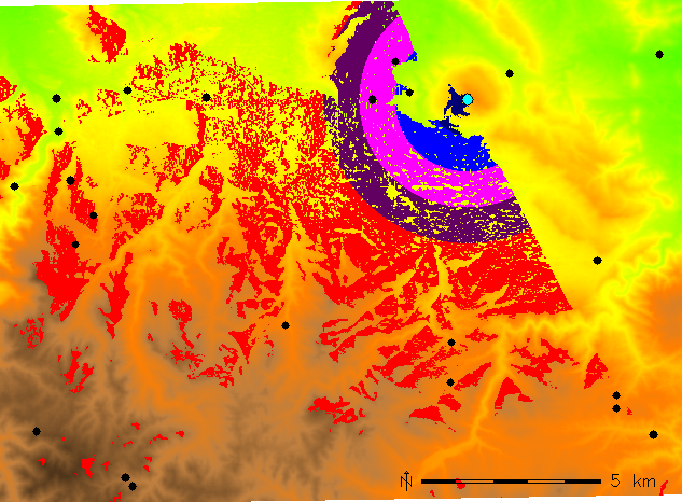
\includegraphics[width=0.7\textwidth]{visibility}
\captionof{figure}{Analisi di vista effettuata con GRASS}
\end{myfig}

\section{Filosofia del software libero}

Il software libero garantisce all'utente l'accesso al codice sorgente assicurandone quindi la trasparenza. Garantisce inoltre il diritto di studiare, estendere, modificare e ridistribuire il codice stesso a patto di garantire gli stessi diritti agli altri utenti. La possibilit\`a di vedere il codice genera un processo di revisione che ne garantisce la qualit\`a. Con l'aiuto dell' "extension manager" si possono inoltre creare nuovi moduli senza dover disporre del pacchetto completo di GRASS.

\section{Scheda tecnica}

\subsection{Licenza}

GNU General Public License (Free Software Foundation)

\subsection{Piattaforme supportate}

GRASS funziona praticamente su ogni piattaforma. In particolare supporta GNU/Linux, Sistemi Unix compatibili con Posix, MS-Windows e MacOS X.

\subsection{Struttura}

\begin{itemize}
\item Modulare con pi\`u di 350 moduli
\end{itemize}

\subsection{Linguaggi di programmazione}

\begin{itemize}
\item ANSI C e interfaccia GRASS- SWIG
\item Python per applicazioni WebGIS
\item versione Java: JGRASS
\end{itemize}

\subsection{Gestione dei dati e potenzialit\`a}

\begin{itemize}
\item processamento di dati Raster / Vettori / Voxel
\item modelli 2D / 3D Raster e Vettoriale 
\item elaborazione immagini, topologia vettoriale ed analisi di reti
\item Geostatistica (interfaccia con R)
\end{itemize}

\begin{myfig}[1ex]
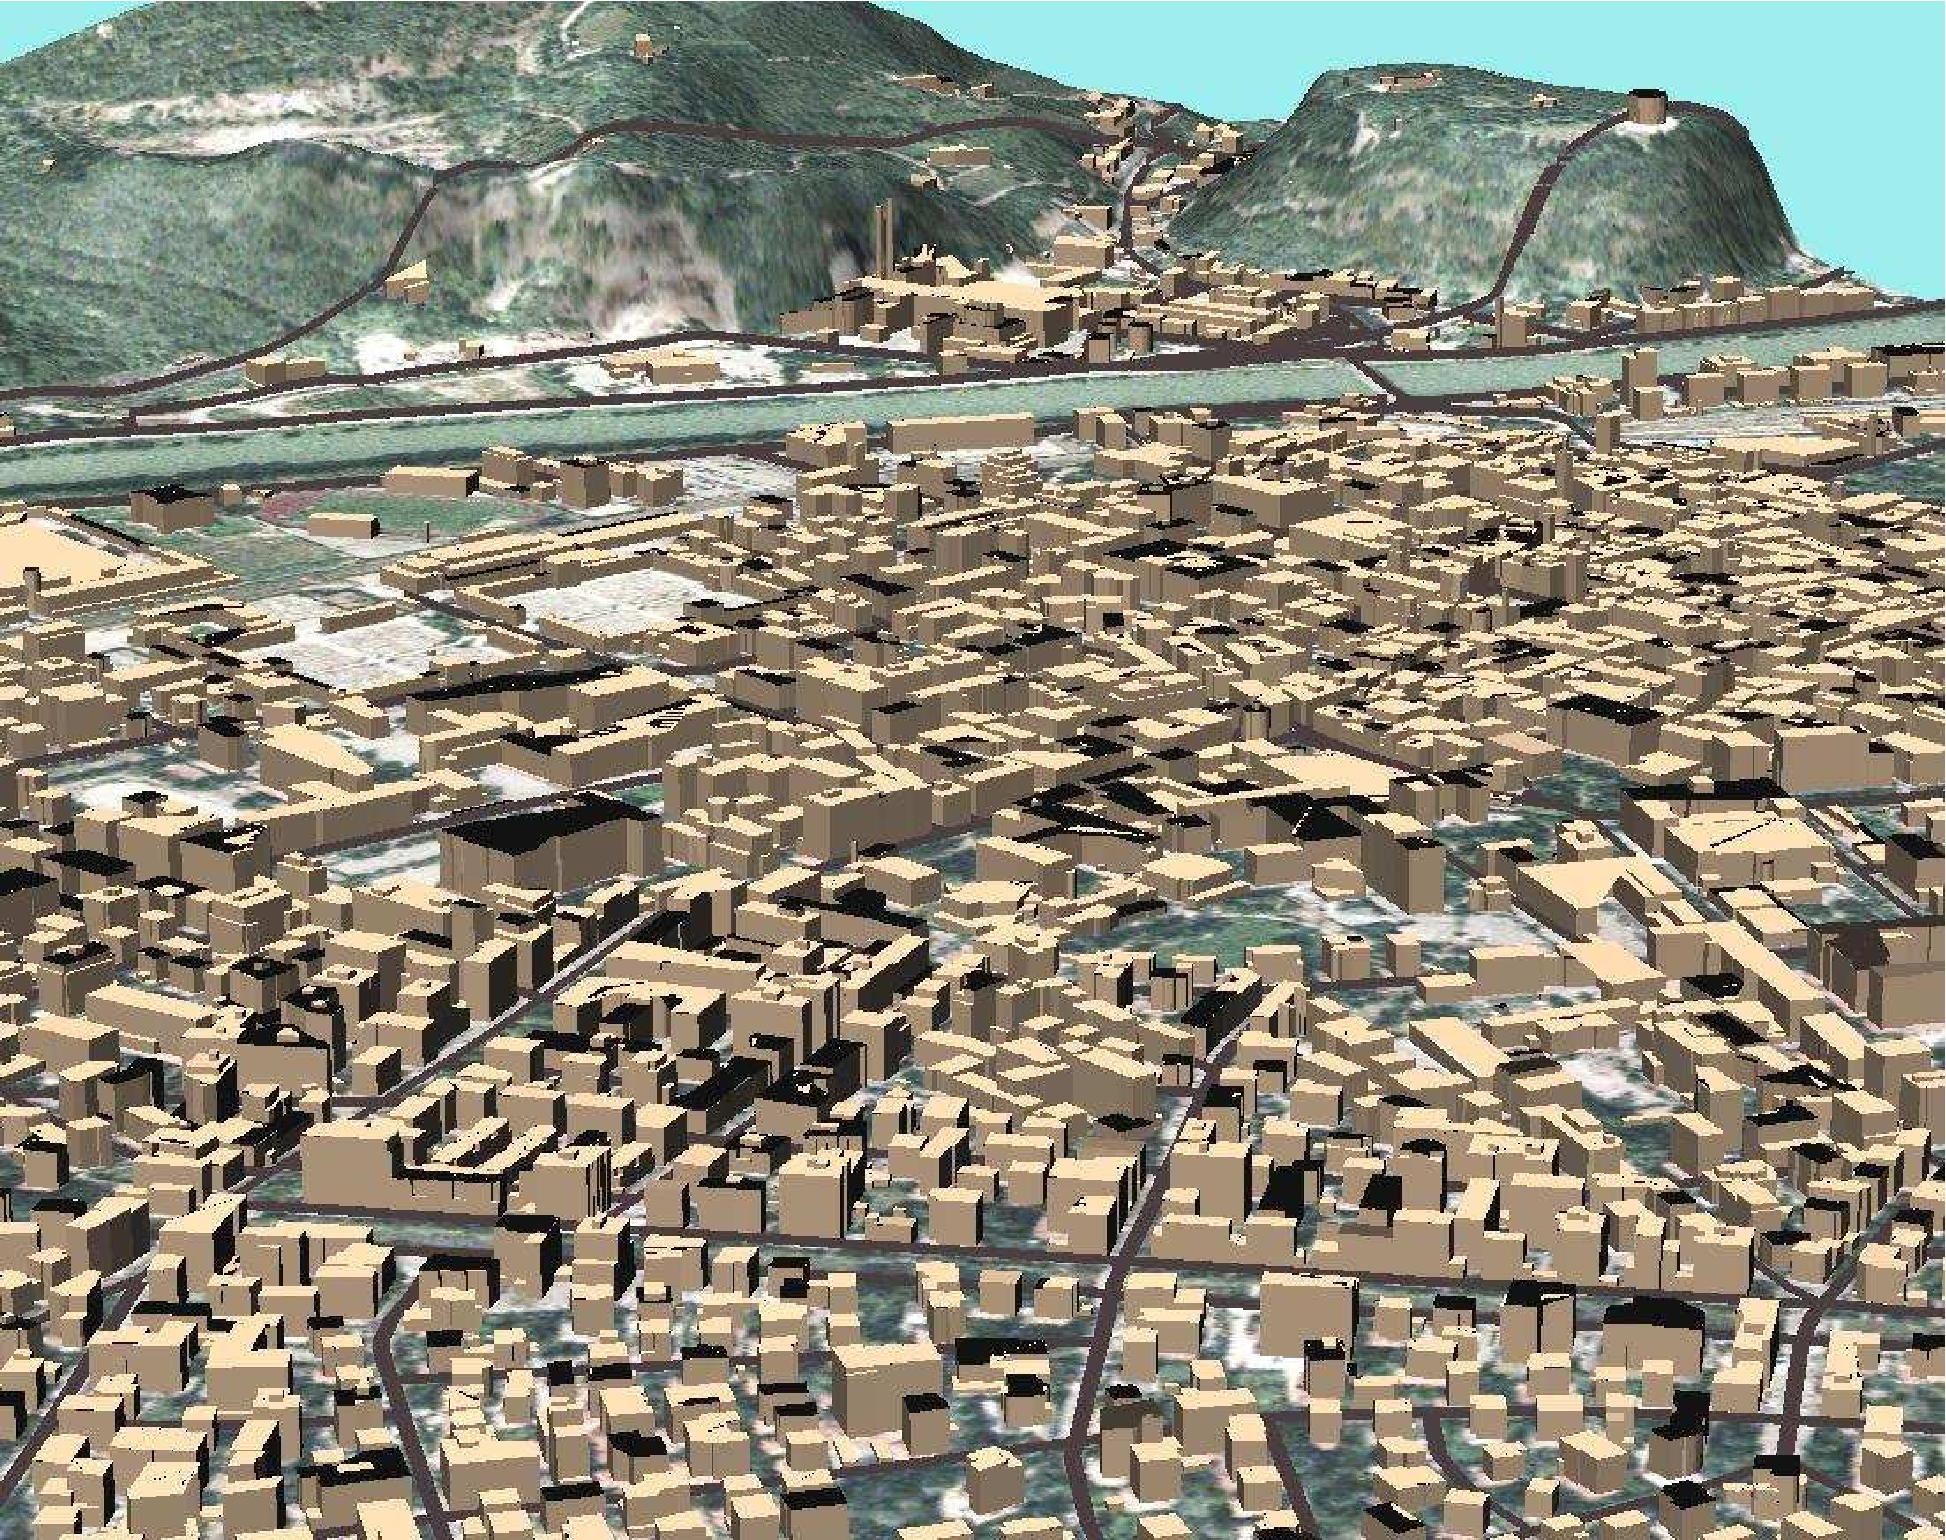
\includegraphics[width=0.7\textwidth]{trento3d}
\captionof{figure}{Vista aerea della citt\`a di Trento}
\end{myfig}

\section{Formati di file supportati}

GRASS supporta tutti i formati di file GIS pi\`u comuni tramite l'utilizzo della libreria GDAL/OGR. Inoltre  supporta lo standard dell'Open GIS Consortium per le Simple Features.

\subsection{Formati di file vettoriali}
ASCII, ARC/INFO, ARC/INFO E00, Arc\-View SHAPE, BIL, DLG (U.S.), DXF, DXF3D, GMT, GPS-ASCII USGS-DEM, IDRISI, MOSS, MapInfo MIF, PostGIS, TIGER, VRML, \dots

\subsection{Formati di file raster}
ASCII, ARC/GRID, E00, GIF, GMT, TIF, PNG, Vis5D, SURFER (.grd),\dots
\begin{myfig}
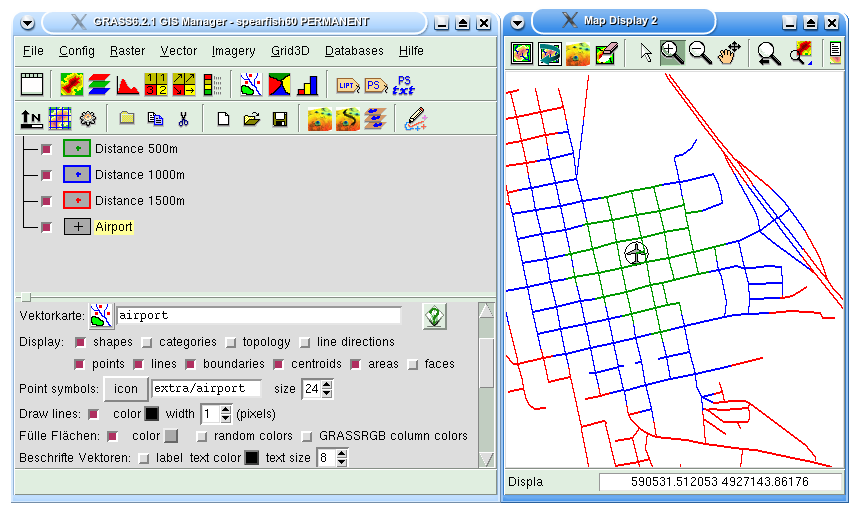
\includegraphics[width=0.7\textwidth]{isodist}
\captionof{figure}{Analisi di reti in GRASS tramite interfaccia grafica}
\end{myfig}

\subsection{Formati di file immagine}

CEOS (SAR, SRTM, LANDSAT7 etc.), ERDAS LAN / IMG, HDF, LANDSAT TM/MSS, NHAP aerial photos, SAR, SPOT, \dots
\begin{myfig}[1.5ex]
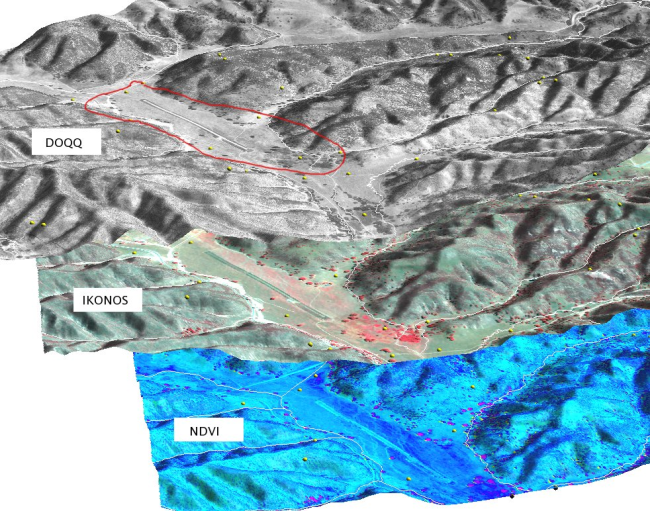
\includegraphics[width=0.7\textwidth]{ndvi}
\captionof{figure}{Analisi d'immagine con GRASS}
\end{myfig}

\subsection{Basi di dati supportate}

\begin{itemize}
\item PostgreSQL / PostGIS
\item MySQL
\item SQLite
\item ODBC
\item DBF
\end{itemize}

\subsection{Output}

\begin{itemize}
\item Moduli per la generazione di mappe
\item NVIZ per la visualizzazione di dati 2.5D e 3D (creazione di animazioni)
%\item{GMT export}
%item{VRML}
\item VTK, POVray
\item WebGIS via Mapserver, Python, etc.
\end{itemize}

\subsection{Interoperabilit\`a con altri GIS ed altri Software}

\begin{itemize}
\item Quantum GIS (Visualizzatore di geodati ed altro)
\item R- Language (Statistica)
\item Gstat (Geostatistica)
\item UMN Mapserver (Webmapping)
\end{itemize}

\section{Dove trovare altre informazioni}

\begin{itemize}
%\begin{flushleft}
\item{Sito Web del progetto [eng]: \\\GRASSurl}
\item{GRASS Wiki  [eng]: \\\url{http://grass.osgeo.org/wiki}}
\item{GRASS Promotion Team  [eng]: \\\url{malte@perlomat.de}}
\item{GRASS mailing lists  [eng]: \\\url{http://grass.osgeo.org/community/support.php}}
\item{Mailing list degli utenti italiani di GRASS  [ita]: \\\url{http://listserv.unipr.it/mailman/listinfo/grass-italia}}
\item{Sito Web degli utenti italiani di GRASS [ita]: \\\url{http://grass-italia.como.polimi.it/}}
%\end{flushleft}
\end{itemize}

\vfill
\section{OSGeo}

GRASS \`e un progetto fondatore dell'Open Source Geospatial Foundation che ha lo scopo di creare software liberi di elevata qualit\`a per la geoscienza. Per ulteriori informazioni visitate il sito di OSGeo:
\begin{center}

\includegraphics[width=0.8\textwidth]{OSGeo_CMYK}\\
\url{http://www.osgeo.org}
\end{center}

\end{document}
